\documentclass[aspectratio=169]{beamer}
\setbeamertemplate{navigation symbols}{}
\usepackage{color,amsmath,comment, subfigure}
\usepackage{booktabs}
\vfill
\usepackage{url}

%%%%%%%%%%%%%%%%%%%%%%%%%%
\title[]{The connected age and the small world problem}
\author[]{Social Networks (Soc 204)\\Spring 2021\\Princeton University}
\institute[]{Matthew J. Salganik}
\date[]{Week 1, Lecture 2\\ Video 2/3: Small world

\vfill

\begin{flushleft}
\vspace{0.7in}

\includegraphics[width=0.05\textwidth]{figures/cc.png}
\end{flushleft}
}

\begin{document}
%%%%%%%%%%%%%%%%%%%%%%%%%%%
\frame{\titlepage}
%%%%%%%%%%%%%%%%%%%%%%%%%%%
\begin{frame}

\begin{center}
\Large{
``Oh my goodness.  It's a small world!''
}
\end{center}

\pause
Two times that people say this:
\begin{itemize}
\item See someone they know in an unexpected place
\pause
\item Meet someone and find out that they have an acquaintance in common
\end{itemize}

\note{
When was the last time you said this?  Think-pair-share.  
Two kinds of experiences. You see someone you know at an expected place.  You 
}

\end{frame}
%%%%%%%%%%%%%%%%%%%%%%%%%%%
\begin{frame}

Let's think back to 1967 . . . . 

\end{frame}
%%%%%%%%%%%%%%%%%%%%%%%%%%%
\begin{frame}

\begin{center}
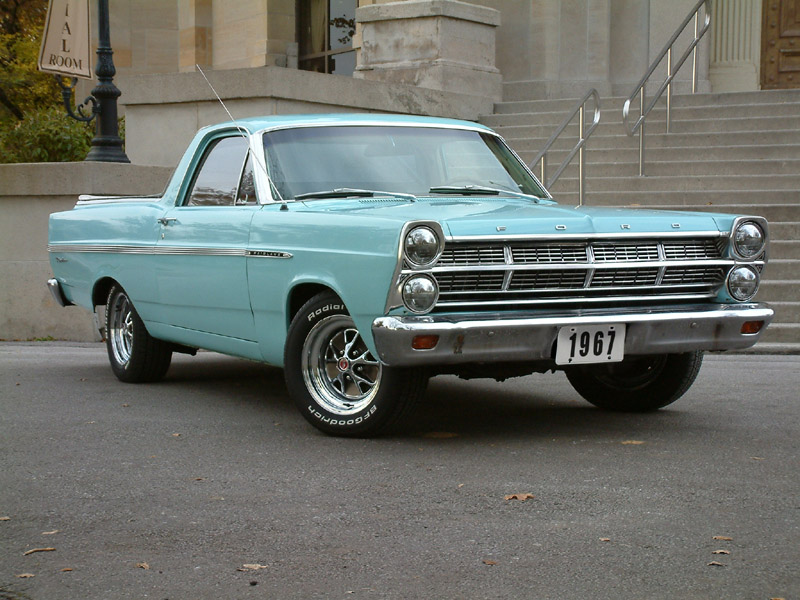
\includegraphics[height=0.8\textheight]{figures/1967_Ford_Fairlane_Ranchero.jpg}
\end{center}

\vfill
\tiny{\url{http://upload.wikimedia.org/wikipedia/commons/f/f5/1967_Ford_Fairlane_Ranchero.jpg}}

\end{frame}
%%%%%%%%%%%%%%%%%%%%%%%%%%%
\begin{frame}

\begin{center}
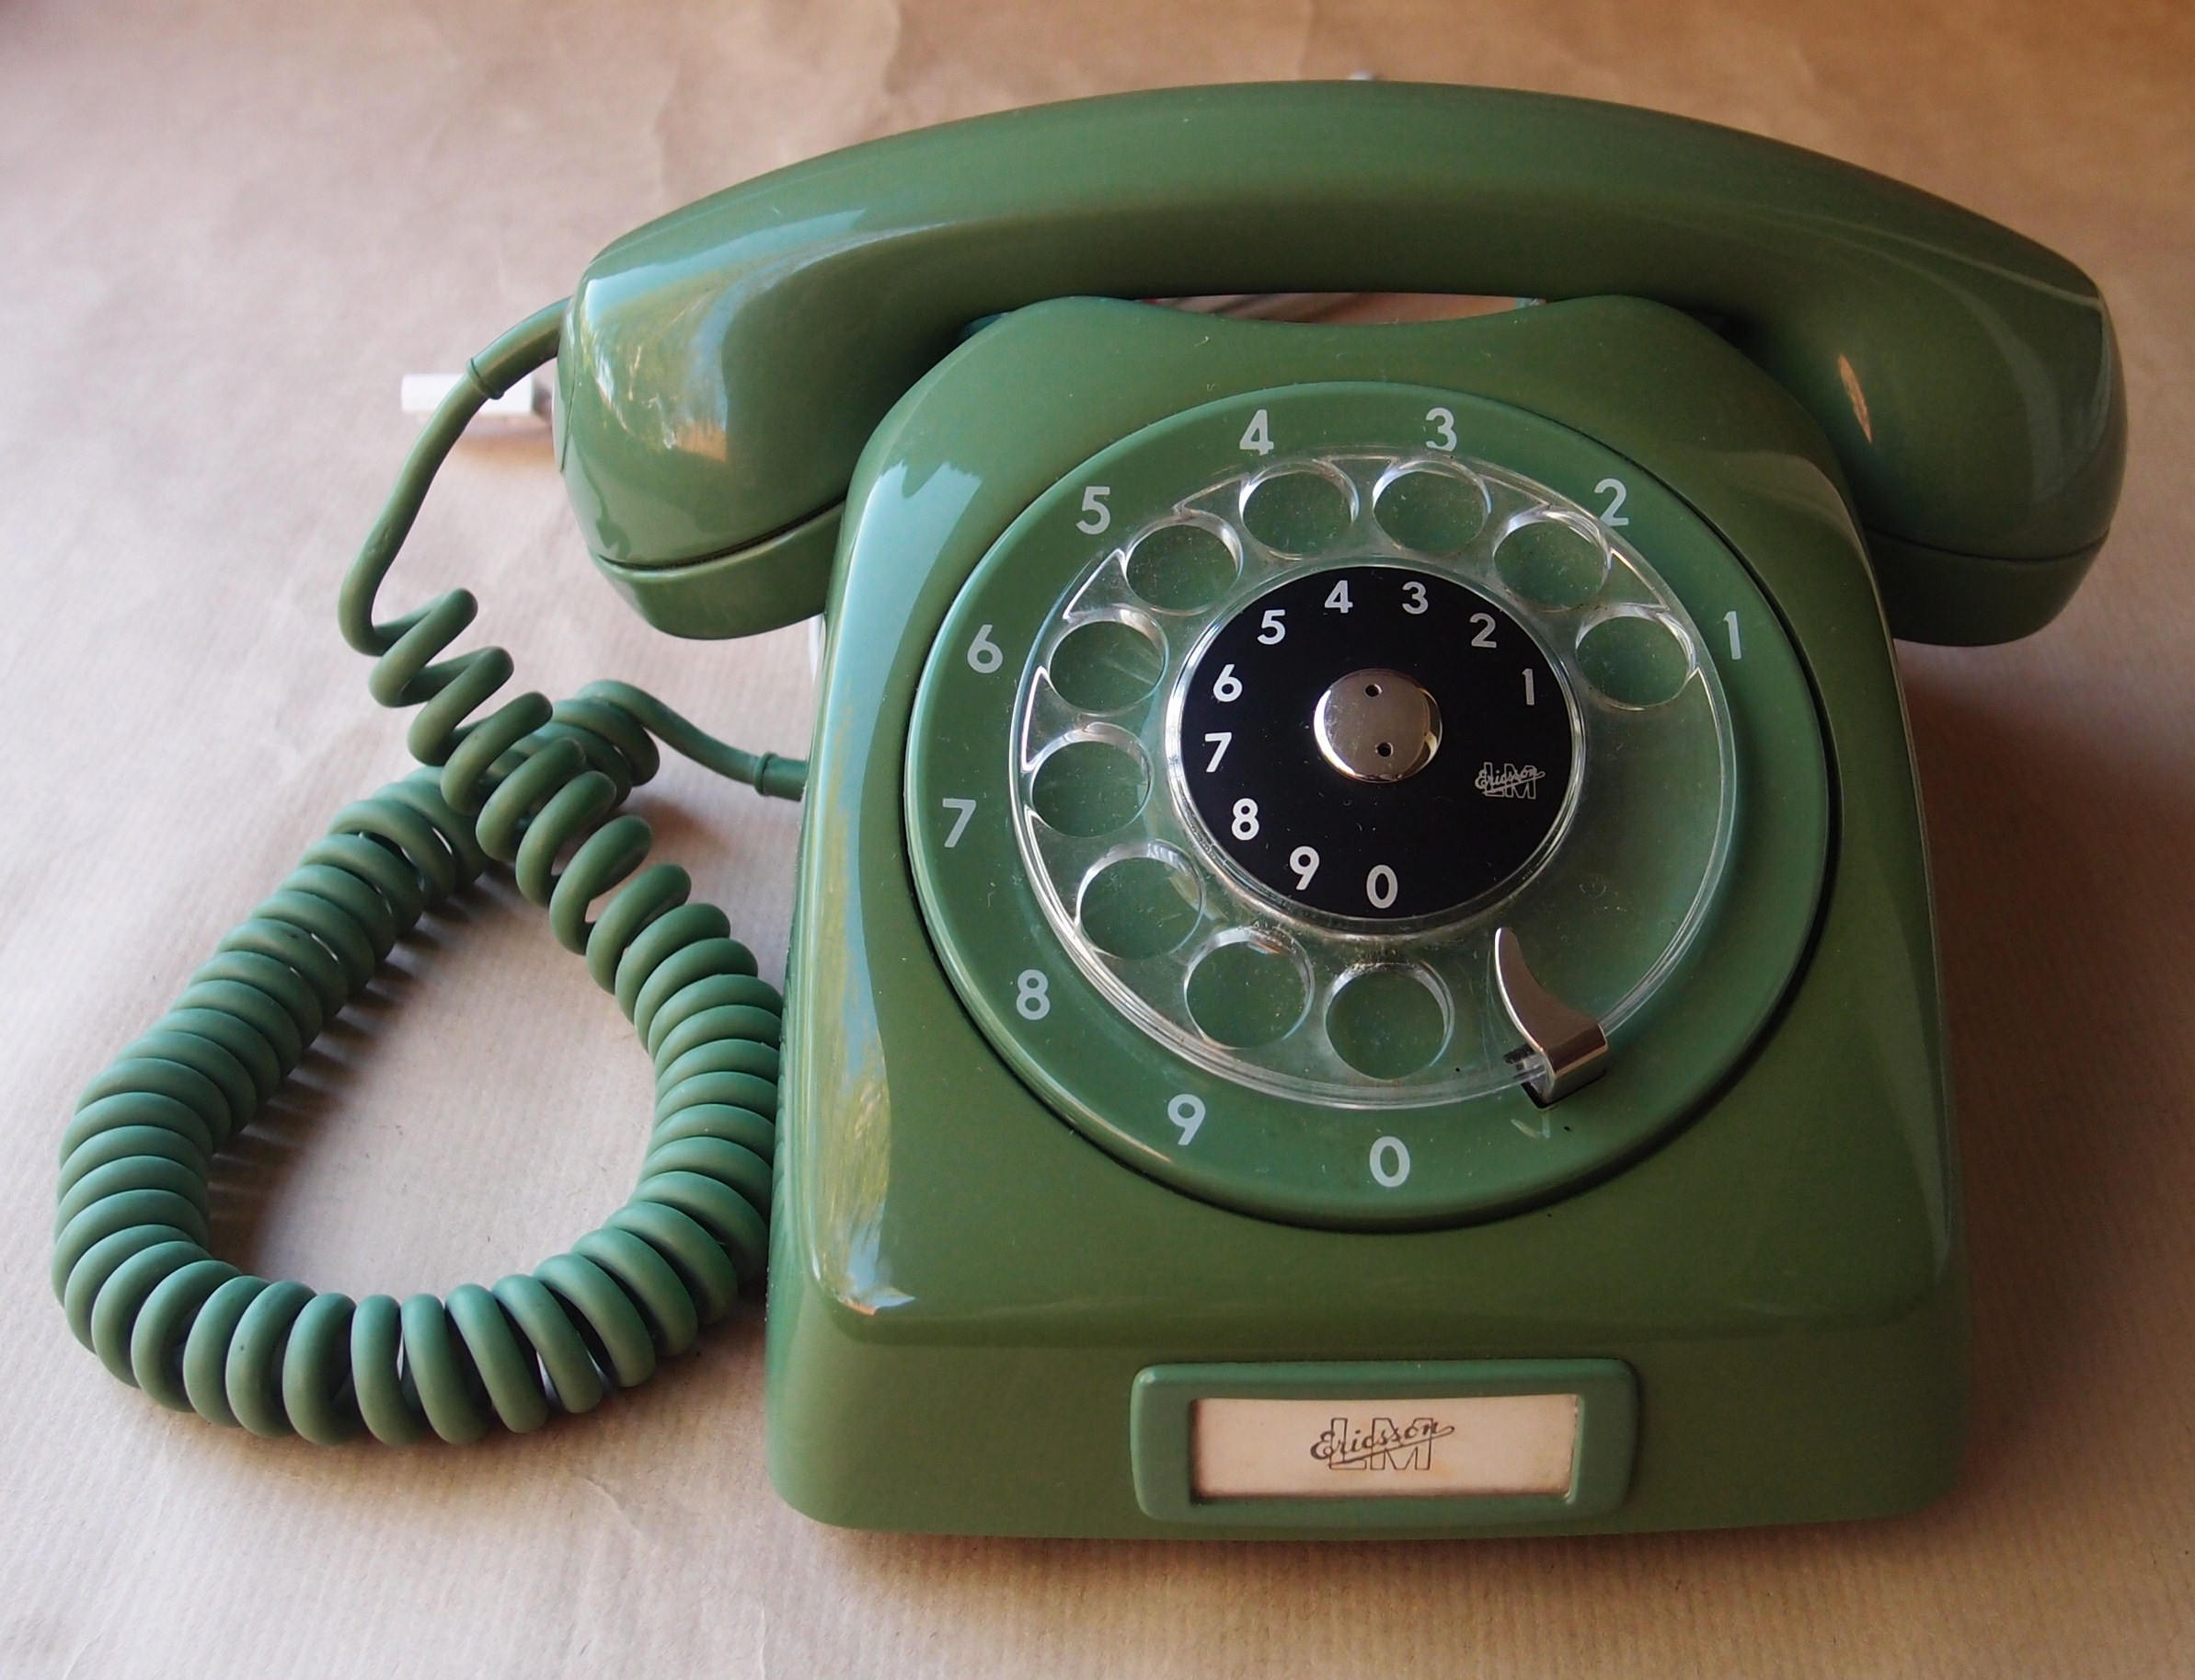
\includegraphics[height=0.8\textheight]{figures/Ericsson_Dialog_in_green}
\end{center}

\vfill
\tiny{\url{http://commons.wikimedia.org/wiki/File:Ericsson_Dialog_in_green.JPG}}

\end{frame}
%%%%%%%%%%%%%%%%%%%%%%%%%%%
\begin{frame}

\begin{center}
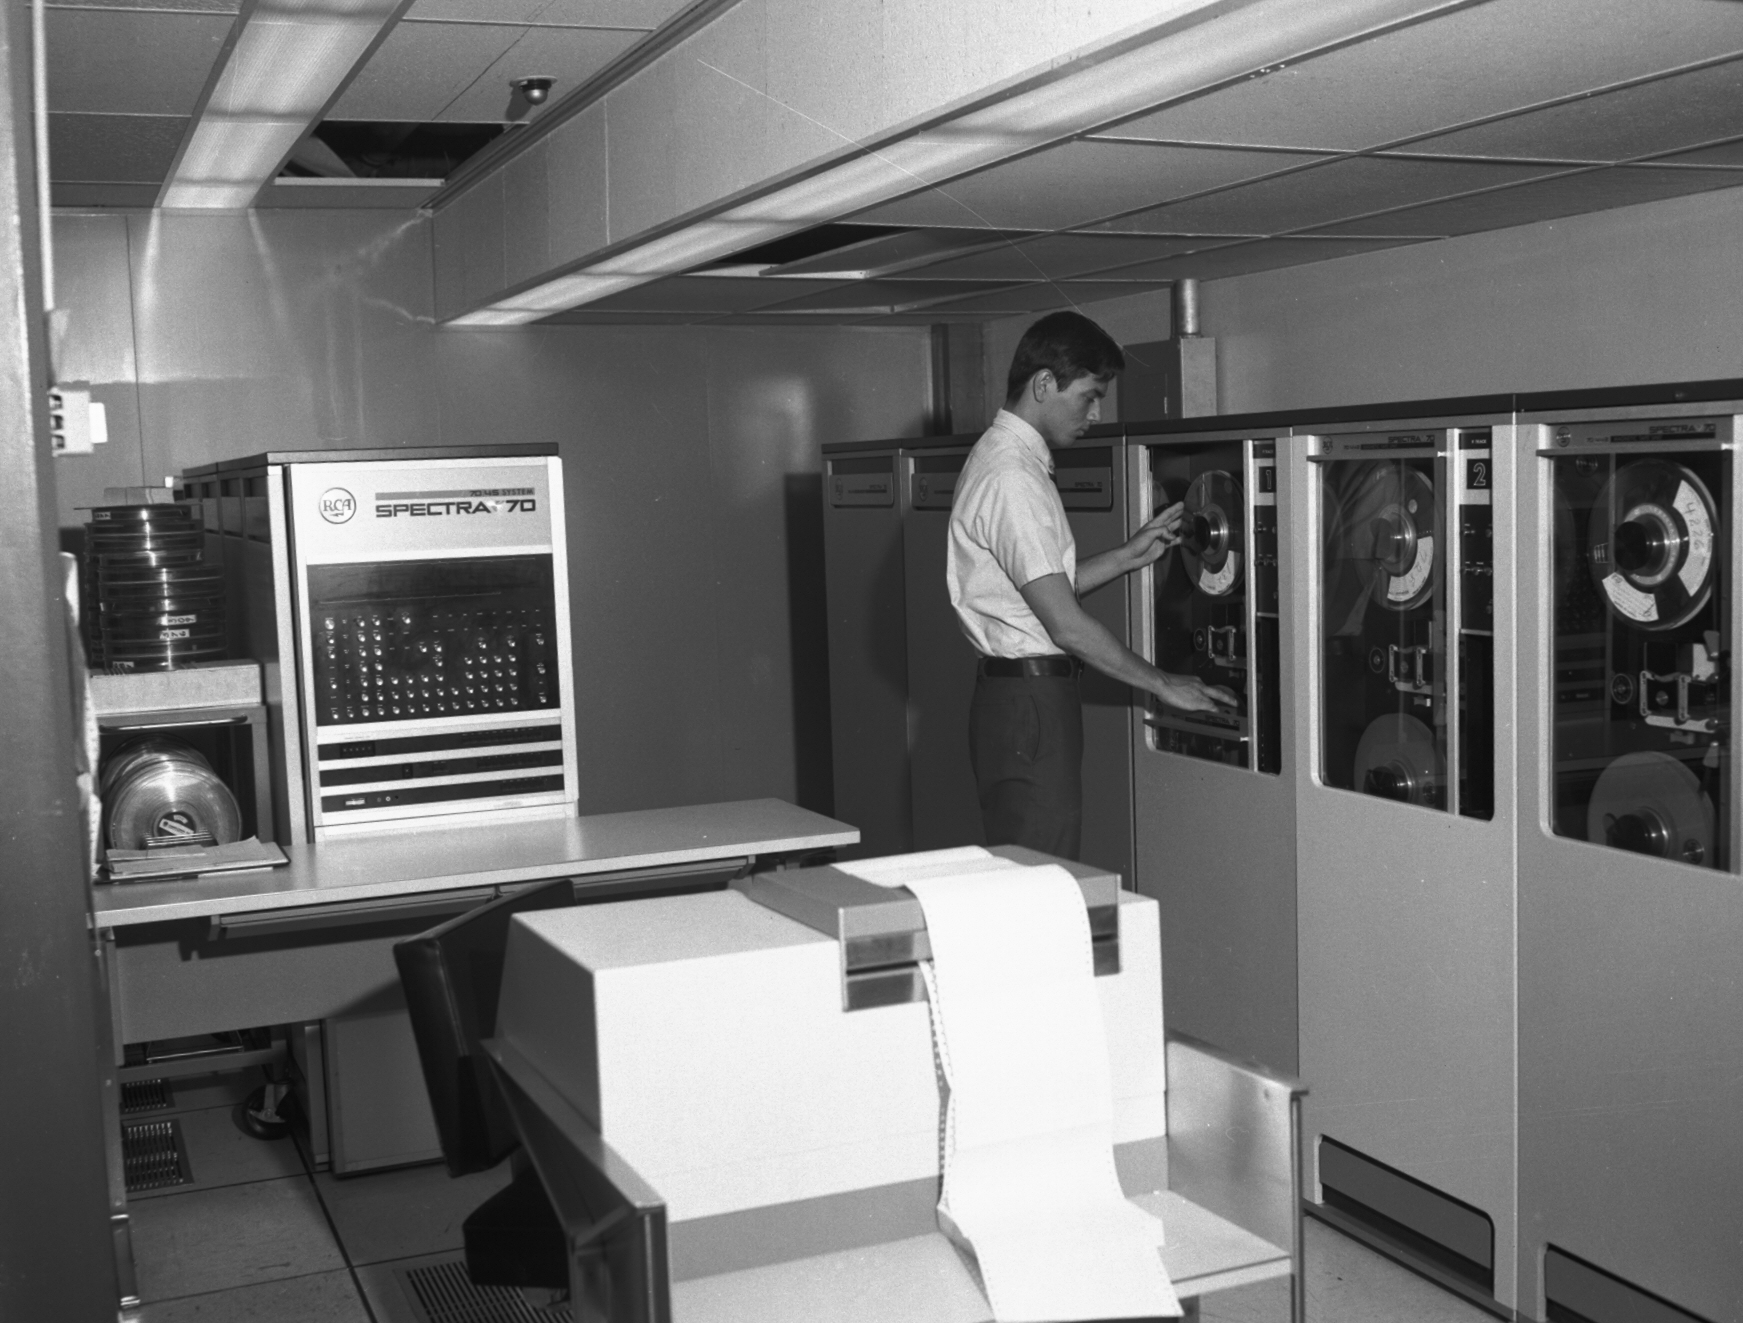
\includegraphics[height=0.8\textheight]{figures/Computer_in_County_of_Orange_offices,_1967}
\end{center}

\vfill
\tiny{\url{http://commons.wikimedia.org/wiki/File:Computer_in_County_of_Orange_offices,_1967.jpg}}

\end{frame}
%%%%%%%%%%%%%%%%%%%%%%%%%%%
\begin{frame}

Fred Jones of Peoria, sitting in a sidewalk cafe in Tunis, and needing a light for his cigarette, asks the man at the next table for a match. They fall into conversation; the stranger is an Englishman who, it turns out, spent several months in Detroit studying the operation of an interchangeable-bottlecap-factory. ``I know it's a foolish question'' says Jones, ``but did you ever by any chance run into a fella named Ben Arkadian? He's an old friend of mine, manages a chain of supermarkets in Detroit . . . '' ``Arkadian, Arkadian'' the Englishman mutters. ``Why, upon my soul, I believe I do! Small chap, very energetic, raised merry hell with the factory over a shipment of defective bottlecaps.'' ``No kidding!'' Jones exclaims in amazement. ``Good lord, it's a small world isn't it!''

\vfill
Milgram (1967)
\end{frame}
%%%%%%%%%%%%%%%%%%%%%%%%%%%
\begin{frame}

\begin{itemize}
\item What is the probability that two people chosen at random know each other?
\pause
\item What is the probability that two people chosen at random share a friend?
\pause
\item Given two individuals selected randomly from the population, what is the probability that the minimum number of intermediaries required to link them is 0,1,2,...k?
\end{itemize}

\end{frame}
%%%%%%%%%%%%%%%%%%%%%%%%%
\begin{frame}

\begin{center}
Modeling approach (i.e., MIT approach)\\
  vs.\\
Empirical approach (i.e., Harvard approach)
\end{center}

\note{
We will see more of the modeling approach next week
}

\end{frame}
%%%%%%%%%%%%%%%%%%%%%%%%%
\begin{frame}

\begin{center}
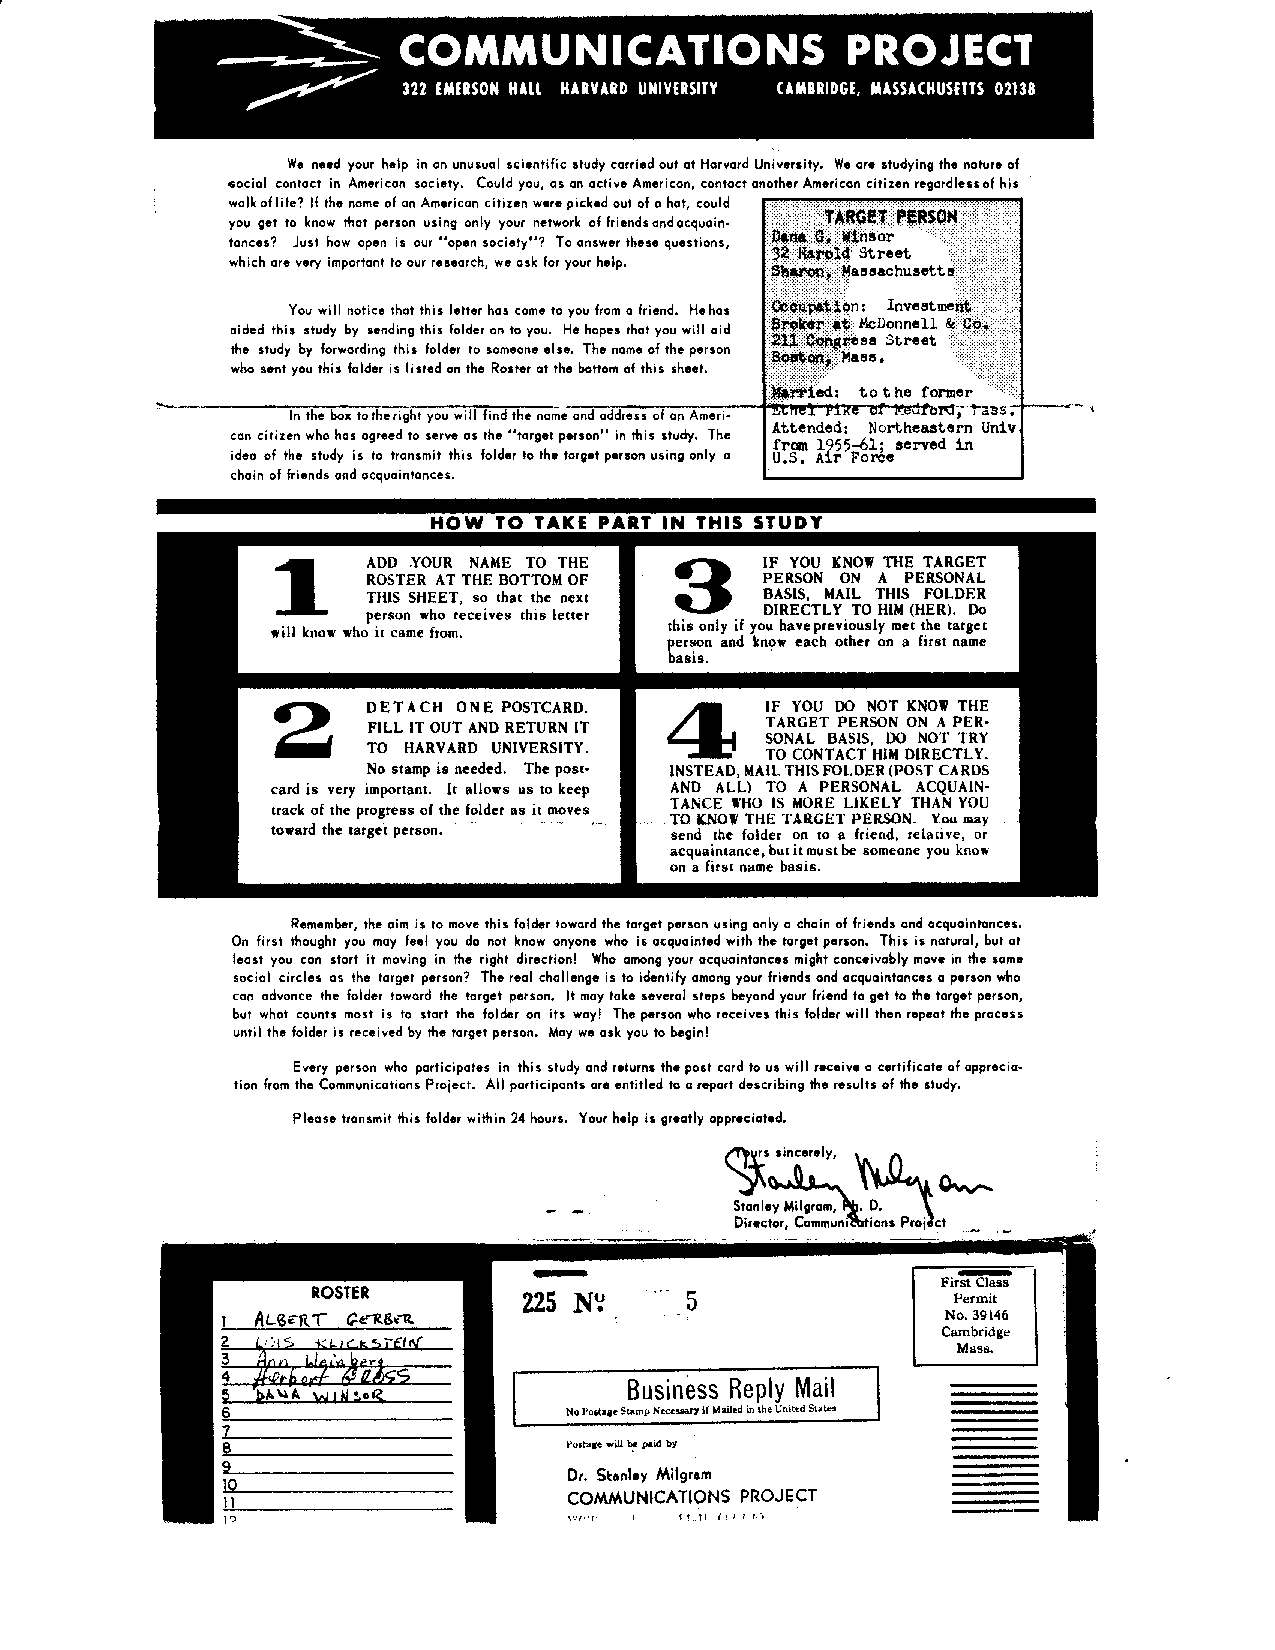
\includegraphics[height=0.9\textheight]{figures/small_world_dossier}
\end{center}

\end{frame}
%%%%%%%%%%%%%%%%%%%%%%%%
\begin{frame}

This procedure is elegant.\pause

\begin{itemize}
\item provides a view of the big invisible social network of Americans
\pause
\item flexible in choice of starters and targets
\pause
\item tracer cards provide data on incomplete chains (and demographics of participants)
\end{itemize}

\note{
flexible in choice of starters
and choice of targets
tracer cards provide data on incomplete chains (and demographics of participants)
also flexible in the type of information provided about the target

There is a big invisible web, and this gives us tracers through it
}

\end{frame}
%%%%%%%%%%%%%%%%%%%%%%%%
\begin{frame}

Results

\end{frame}
%%%%%%%%%%%%%%%%%%%%%%%%%
\begin{frame}
\frametitle{Result 1}

\begin{center}
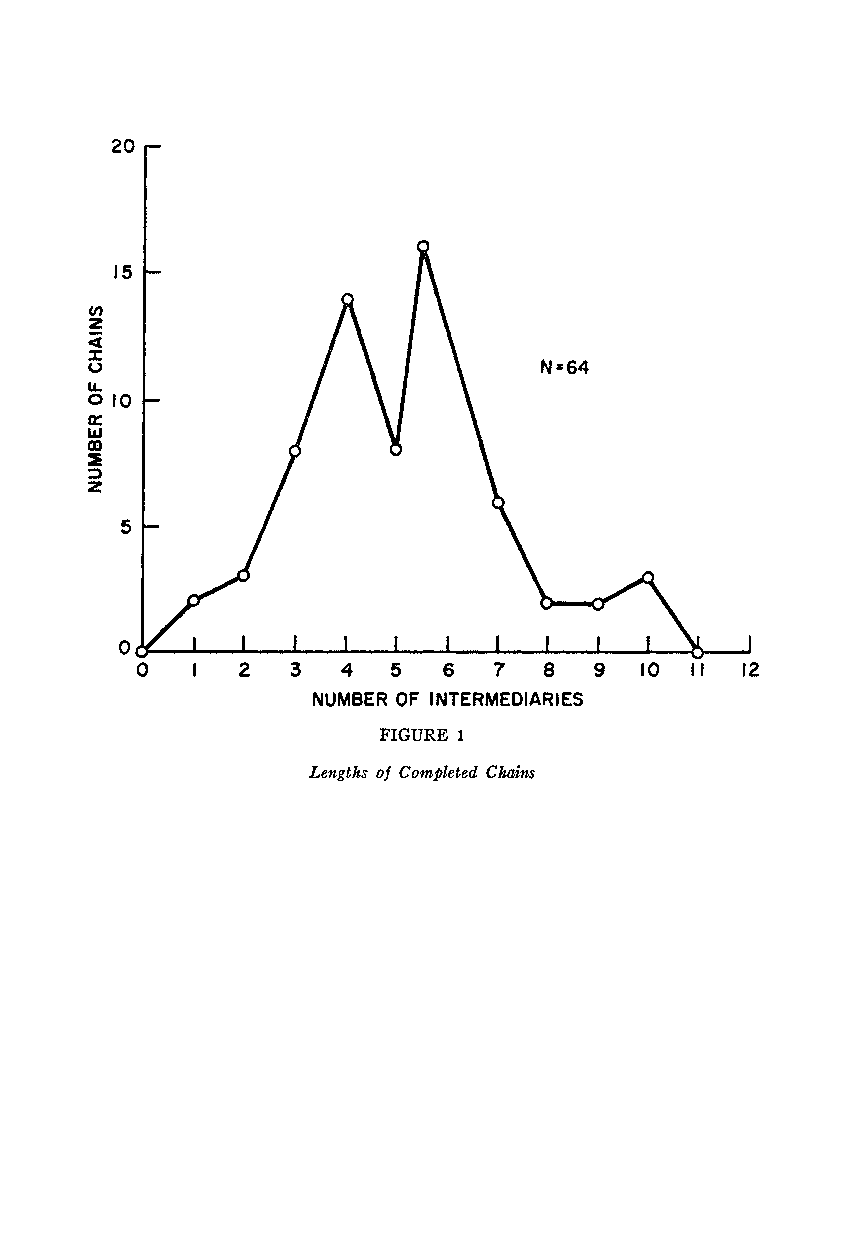
\includegraphics[height=0.7\textheight]{figures/travers_experimental_1969_fig1}
\end{center}

Mean number of intermediaries: 5.2\\ 

\end{frame}
%%%%%%%%%%%%%%%%%%%%%%%%%%%
\begin{frame}
\frametitle{Result 1}

\begin{itemize}
\item 1 intermediary = 2 ``degrees of separation''
\pause
\item 5 intermediaries = 6 ``degrees of separation''
\end{itemize}

\end{frame}
%%%%%%%%%%%%%%%%%%%%%%%%%%%
\begin{frame}
\frametitle{Result 2}

\begin{itemize}
\item Travers and Milgram: 29\% of chains reached target
\pause
\item Kleinfeld: 71\% of chains did not reach target
\end{itemize}

\pause
Be careful as you read.

\note{
scientists call attention to make their work look good (similar to politicians)
folder demo
more likely to see short chains than long chains
}

\end{frame}
%%%%%%%%%%%%%%%%%%%%%%%%%%%
\begin{frame}
\frametitle{Result 3}

\begin{center}
\includegraphics<1>[height=0.6\textheight]{figures/travers_experimental_1969_tab2b}
\end{center}

\note{
What does this design reveal about Milgram?
Anyone here from Nebraska
}

\end{frame}
%%%%%%%%%%%%%%%%%%%%%%%%%%%
\begin{frame}
\frametitle{Result 4}

\begin{center}
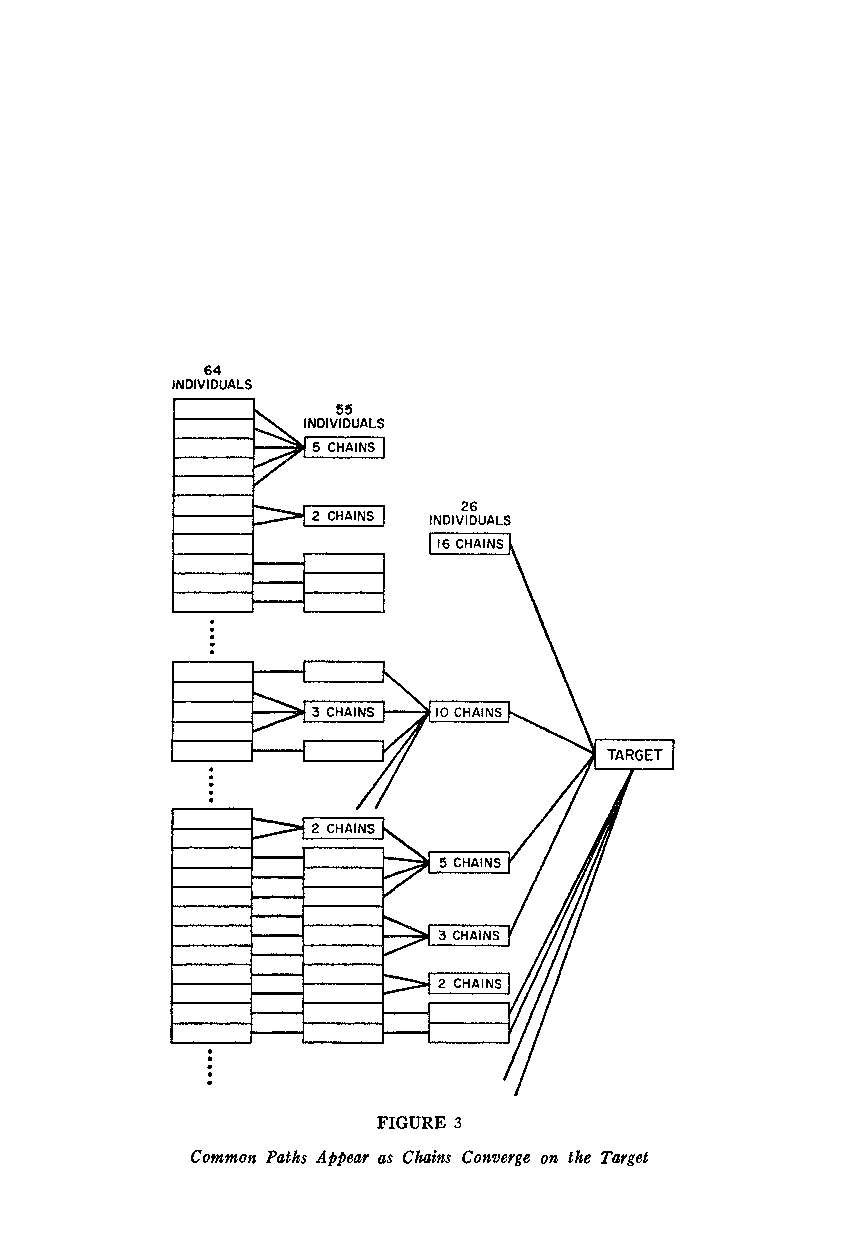
\includegraphics[height=0.9\textheight]{figures/travers_experimental_1969_fig3}
\end{center}


\end{frame}
%%%%%%%%%%%%%%%%%%%%%%%%%
\begin{frame}
\frametitle{Result 4}

\begin{center}
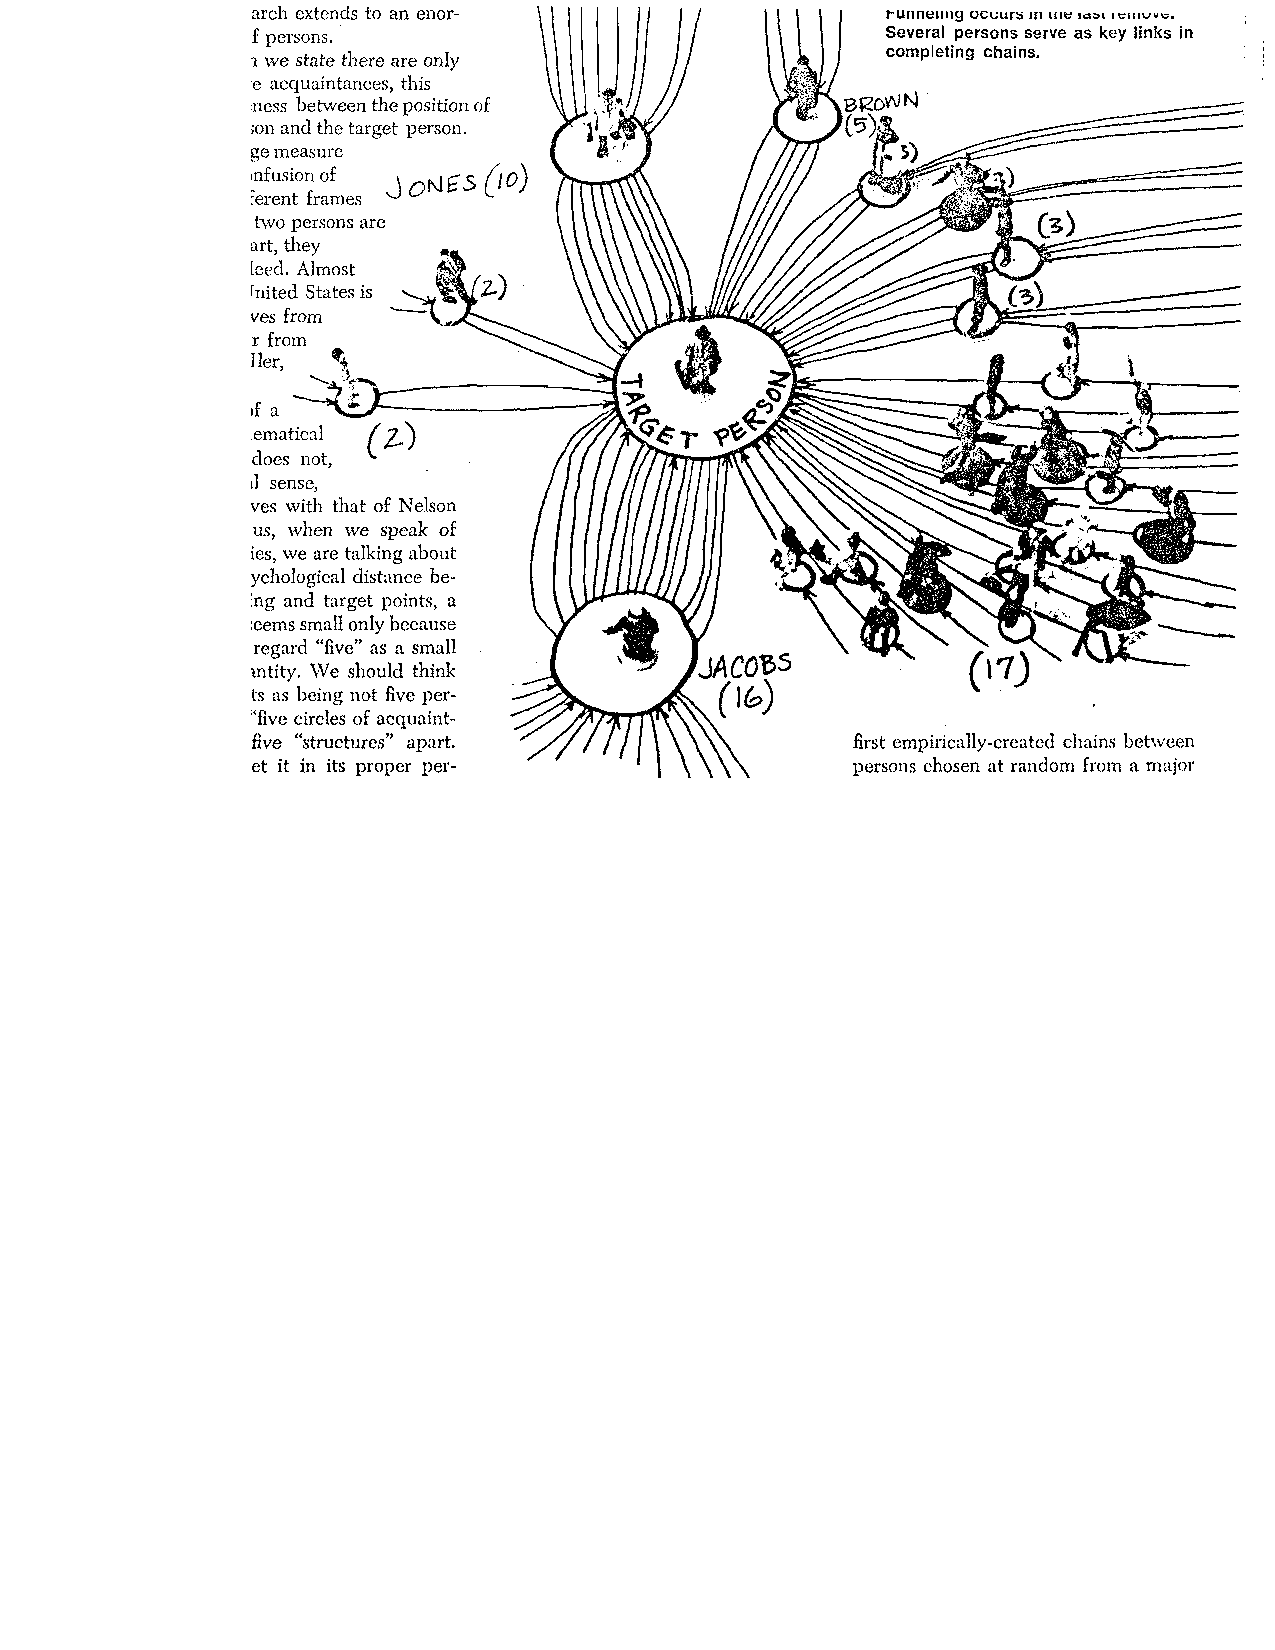
\includegraphics[height=0.8\textheight]{figures/milgram_small-world_1967_funneling}
\end{center}

Funneling, will be the subject of future work

\end{frame}
%%%%%%%%%%%%%%%%%%%%%%%%%
\begin{frame}
\frametitle{}

This is just one of many possible small world experiments. Milgram choose to do others. Let's see what he did. . .

\end{frame}
%%%%%%%%%%%%%%%%%%%%%%%%%


\end{document}
